\section{乘子条件}
\label{sec:kkt-multipliers}

到目前为止，局部最小点的必要条件是“线性化锥中没有下降方向”，前提是线性化准确。这句话要对无穷多个方向逐一检验，不便于计算。接下来要弄清：怎样把它改写成有限个关于梯度的方程？先看只有等式约束的情形，再加入不等式，最后回答这组方程何时必要、何时充分。

\subsection{等式约束的Lagrange乘子}
\label{sec:kkt-lagrange}

下面的问题足够小，可以用三种办法解，比较它们就能看出乘子从哪里来：
\begin{equation}
 \min_{\bm{x}\in\mathbb{R}^2}\ \frac12(x_1^2+4x_2^2)\quad\text{s.t.}\quad x_1+x_2=1.
 \label{eq:kkt-equality-qp}
\end{equation}

\paragraph{第一种办法：消去约束}
可行集是一条直线，用参数$s$表示为$\bm{x}(s)=(1-s,s)$。把它代入目标，就成了无约束的一元问题：
\[
 \phi(s)=\frac12\bigl[(1-s)^2+4s^2\bigr],\qquad\phi'(s)=5s-1.
\]
令导数为零，得$s=1/5$。于是
\[
 \bm{x}^\star=\Bigl(\frac45,\frac15\Bigr),\qquad f^\star=\frac12\Bigl(\frac{16}{25}+\frac{4}{25}\Bigr)=\frac25.
\]
$\phi''=5>0$，这是一元凸二次函数的最小点，所以$\bm{x}^\star$是全局最小点。

\paragraph{第二种办法：切向导数为零}
由链式法则，$\phi'(s)$就是梯度沿直线方向$\bm{v}=(-1,1)$的方向导数：
\[
 \phi'(s)=\langle\nabla f(\bm{x}(s)),\bm{v}\rangle=-x_1+4x_2.
\]
令它为零，再加上$x_1+x_2=1$，解出同样的点。这说明最优点的条件是：梯度在约束直线的切向上没有分量。

\paragraph{第三种办法：梯度平行于法向}
切向分量为零，就是说梯度垂直于直线，也就是平行于约束的法向$\nabla h=(1,1)$。在$\bm{x}^\star$处，
\[
 \nabla f(\bm{x}^\star)=\Bigl(\frac45,\frac45\Bigr)=\frac45\,\nabla h(\bm{x}^\star).
\]
把这个比例系数写成$-\nu$，关系就成了$\nabla f+\nu\nabla h=\bm{0}$，这里$\nu=-4/5$。这个系数称为\term{Lagrange乘子}（Lagrange multiplier）。

反过来也能从方程解。未知量是$x_1,x_2,\nu$，方程是
\[
 x_1+\nu=0,\qquad 4x_2+\nu=0,\qquad x_1+x_2=1.
\]
前两式给出$x_1=-\nu$，$x_2=-\nu/4$，代入第三式得$-\frac54\nu=1$，于是$\nu=-4/5$，点仍是$(4/5,1/5)$。这个方程组对任意光滑问题都能写出来，不需要先把约束参数化。

图~\ref{fig:kkt-equality-tangency}(a)是这件事的几何。最优点处直线与一条等高线相切，所以两者法向平行。在非最优的可行点$\bar{\bm{x}}=(0.2,0.8)$，梯度$(0.2,3.2)$不垂直于直线，它沿$\bm{v}$的分量给出$\phi'(0.8)=3$，与图(b)中的斜率相同，反向移动（绿色箭头）就能下降。

\begin{BookInlineFigure}
  \centering
  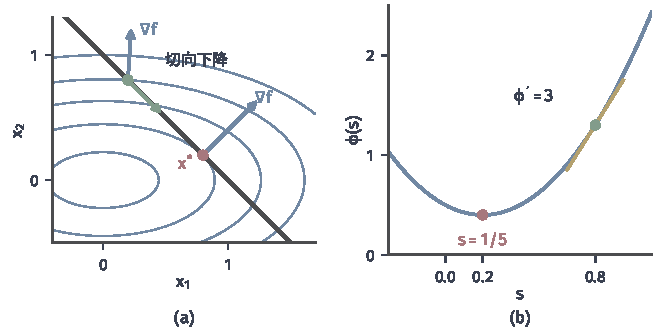
\includegraphics[width=112mm]{figures/05-optimization/06-constrained-optimization/matplotlib/kkt-equality-tangency/figure.pdf}
  \caption{等式约束问题~\eqref{eq:kkt-equality-qp}的切点条件。(a)蓝线是目标的等高线，深灰线是约束直线。红点$\bm{x}^\star=(4/5,1/5)$处直线与等高线相切，梯度沿法向。绿点$(0.2,0.8)$处梯度有切向分量，绿色箭头是沿直线的下降方向。(b)目标沿直线的限制$\phi(s)=f(1-s,s)$，红点是最小点$s=1/5$，绿点$s=0.8$处的切线（黄色）斜率为$3$。}
  \label{fig:kkt-equality-tangency}
\end{BookInlineFigure}

一般的等式约束情形完全一样，只是切向从一条线变成一个子空间。

\begin{theorem}[等式约束的一阶必要条件]
\label{thm:kkt-lagrange}
考虑只有等式约束的问题~\eqref{eq:kkt-problem}（$m=0$）。设$f$、$h_j$在局部最小点$\bm{x}^\star$附近连续可微，$\nabla h_1(\bm{x}^\star),\ldots,\nabla h_p(\bm{x}^\star)$线性无关。则存在唯一的$\bm{\nu}^\star\in\mathbb{R}^p$，使
\begin{equation}
 \nabla f(\bm{x}^\star)+\sum_{j=1}^p\nu_j^\star\nabla h_j(\bm{x}^\star)=\bm{0}.
 \label{eq:kkt-lagrange}
\end{equation}
\end{theorem}

\begin{proof}
以$\nabla h_j(\bm{x}^\star)^\top$为行组成矩阵$\bm{E}$。由定理~\ref{thm:kkt-licq-exact}，切锥等于线性化锥。这里线性化锥就是$\bm{E}$的零空间，是一个子空间。

由定理~\ref{thm:kkt-tangent-necessary}，对这个子空间中的$\bm{d}$有$\langle\nabla f(\bm{x}^\star),\bm{d}\rangle\geq0$。$-\bm{d}$也在子空间内，所以内积只能为零，即$\nabla f(\bm{x}^\star)$与$\bm{E}$的零空间正交。

零空间的正交补是$\bm{E}^\top$的值域，所以存在$\bm{u}$使$\nabla f(\bm{x}^\star)=\bm{E}^\top\bm{u}$，令$\bm{\nu}^\star=-\bm{u}$即得式~\eqref{eq:kkt-lagrange}。唯一性来自$\bm{E}^\top$的列线性无关。
\end{proof}

把目标和约束按乘子加权相加，定义\term{Lagrange函数}（Lagrangian）
\begin{equation}
 \mathcal{L}(\bm{x},\bm{\nu})=f(\bm{x})+\sum_{j=1}^p\nu_jh_j(\bm{x}).
 \label{eq:kkt-lagrangian-equality}
\end{equation}
式~\eqref{eq:kkt-lagrange}就是$\nabla_{\bm{x}}\mathcal{L}=\bm{0}$在$(\bm{x}^\star,\bm{\nu}^\star)$处成立，可行性$h_j=0$就是$\nabla_{\bm{\nu}}\mathcal{L}=\bm{0}$。约束问题的一阶条件由此写成了无约束形式的驻定方程。要注意，这只是驻定，$\mathcal{L}$在$\bm{x}^\star$不必取最小值，更不是在$(\bm{x},\bm{\nu})$上取最小值。

乘子还有一层经济含义。把例子的约束放松成$x_1+x_2=1+\varepsilon$，同样的计算给出最优值$\frac25(1+\varepsilon)^2$，它在$\varepsilon=0$处的导数是$4/5=-\nu$。所以$\lvert\nu\rvert$是约束右端变动一个单位时最优值的变化率，这叫影子价格。这里只是在一个例子上观察，一般结论和条件由第~\ref{chap:parametric-sensitivity}章讨论。

\subsection{不等式约束的KKT条件}
\label{sec:kkt-conditions}

等式约束的切向是子空间，$\bm{d}$和$-\bm{d}$都能走，所以乘子的符号不受限制。不等式只限制朝外的一侧，切向变成了锥，乘子应该带上符号。先用预算例看看符号是怎么来的。

\paragraph{力的平衡}
把$-\nabla f$想成目标施加在点上的拉力，把活动约束想成一堵墙。墙只能把点往内推，不能把点往外拉，第$i$堵墙的推力沿内法向，写成$-\lambda_i\nabla g_i$，其中$\lambda_i\geq0$是推力大小。不活动的约束碰不到点，推力为零。点在最优位置保持不动，意味着合力为零：
\begin{equation}
 -\nabla f(\bm{x}^\star)=\sum_{i\in A(\bm{x}^\star)}\lambda_i\nabla g_i(\bm{x}^\star),\qquad\lambda_i\geq0.
 \label{eq:kkt-force-balance}
\end{equation}
这个类比只解释一阶平衡，它不涉及动力学或曲率。等式约束是两面都有墙的轨道，推力可正可负，所以乘子不限号。

图~\ref{fig:kkt-force-balance}算了两个例子。$\tau=2$时只有预算线活动，$-\nabla f=(1/2,1/2)$，一堵墙就够了：$\lambda_1=1/2$。$\tau=1/2$时最优点在角点，两堵墙合力，由
\[
 \Bigl(\frac32,1\Bigr)=\lambda_1(1,1)+\lambda_3(0,-1)
\]
解出$\lambda_1=3/2$，$\lambda_3=1/2$，都非负。

\begin{BookInlineFigure}
  \centering
  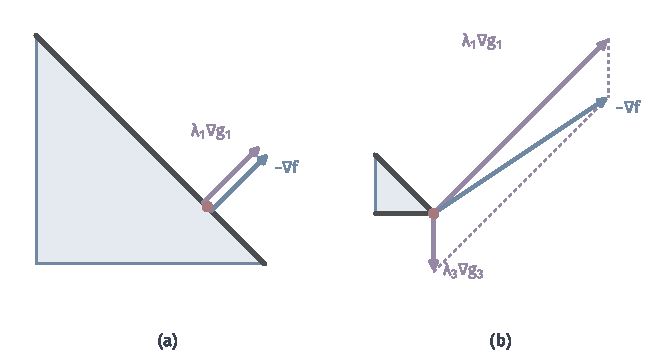
\includegraphics[width=112mm]{figures/05-optimization/06-constrained-optimization/matplotlib/kkt-force-balance/figure.pdf}
  \caption{最优点处的力的平衡。蓝色箭头是负梯度，紫色箭头是$\lambda_i\nabla g_i$。(a)$\tau=2$：$-\nabla f=\frac12\nabla g_1$（两箭头实际重合，为看清而错开绘制）。(b)$\tau=1/2$：$-\nabla f=\frac32\nabla g_1+\frac12\nabla g_3$，虚线组成平行四边形。}
  \label{fig:kkt-force-balance}
\end{BookInlineFigure}

\paragraph{从无下降方向到乘子}
力的平衡是直观，严格的推导要用第~\ref{chap:linear-programming}章的Farkas引理：对矩阵$\bm{M}$和向量$\bm{b}$，系统$\bm{M}\bm{u}=\bm{b}$，$\bm{u}\geq\bm{0}$与系统$\bm{M}^\top\bm{z}\geq\bm{0}$，$\bm{b}^\top\bm{z}<0$恰有一个有解。几何上，$\bm{b}$要么在$\bm{M}$的列张成的锥内，要么能被一个超平面与锥隔开。

\begin{lemma}[无线性化下降方向与乘子]
\label{lem:kkt-farkas}
设$\bar{\bm{x}}\in\bm{C}$，$f$与约束函数在$\bar{\bm{x}}$处可微。不存在$\bm{d}\in\bm{F}(\bar{\bm{x}})$使$\langle\nabla f(\bar{\bm{x}}),\bm{d}\rangle<0$，当且仅当存在$\lambda_i\geq0$（$i\in A(\bar{\bm{x}})$）和$\nu_j\in\mathbb{R}$，使
\begin{equation}
 \nabla f(\bar{\bm{x}})+\sum_{i\in A(\bar{\bm{x}})}\lambda_i\nabla g_i(\bar{\bm{x}})+\sum_{j=1}^p\nu_j\nabla h_j(\bar{\bm{x}})=\bm{0}.
 \label{eq:kkt-farkas-stationary}
\end{equation}
\end{lemma}

\begin{proof}
以活动的$\nabla g_i(\bar{\bm{x}})^\top$为行组成$\bm{B}$，以$\nabla h_j(\bar{\bm{x}})^\top$为行组成$\bm{E}$，在Farkas引理中取
\[
 \bm{M}=\begin{bmatrix}\bm{B}^\top&\bm{E}^\top&-\bm{E}^\top\end{bmatrix},\qquad\bm{b}=-\nabla f(\bar{\bm{x}}).
\]
把等式乘子拆成$\bm{\nu}=\bm{\nu}^{+}-\bm{\nu}^{-}$，两部分都非负，并记
\[
 \bm{u}=(\bm{\lambda}_A,\bm{\nu}^{+},\bm{\nu}^{-})\geq\bm{0},
\]
其中$\bm{\lambda}_A$是活动约束的乘子。方程$\bm{M}\bm{u}=\bm{b}$正是式~\eqref{eq:kkt-farkas-stationary}。

另一个系统要求$\bm{B}\bm{z}\geq\bm{0}$，$\bm{E}\bm{z}=\bm{0}$，$\langle\nabla f(\bar{\bm{x}}),\bm{z}\rangle>0$。令$\bm{d}=-\bm{z}$，它等价于
\[
 \bm{B}\bm{d}\leq\bm{0},\qquad\bm{E}\bm{d}=\bm{0},\qquad\langle\nabla f(\bar{\bm{x}}),\bm{d}\rangle<0,
\]
即存在线性化下降方向。Farkas引理说两个系统恰有一个有解，这就是要证的等价。
\end{proof}

图~\ref{fig:kkt-farkas-cone}画出引理的两种情形，两张图的约束梯度相同。(a)是$\tau=1/2$的角点，$-\nabla f$落在紫色的梯度锥内，乘子存在，绿色的线性化锥与它成钝角，没有下降方向。(b)是$\tau=2$时的角点$(2,0)$，这一点可行但不是最优点。这里$-\nabla f=(0,1)$在锥外。

解驻定方程$(0,-1)+\lambda_1(1,1)+\lambda_3(0,-1)=\bm{0}$，得$\lambda_1=0$，$\lambda_3=-1$，符号不对。负乘子正好指出了下降方向$\bm{d}=(-1,1)$，也就是离开$x_2=0$这堵墙：
\[
 f(2-s,s)=\frac12\bigl[s^2+(1-s)^2\bigr],\qquad\frac{\mathrm{d}}{\mathrm{d}s}f\Big|_{s=0}=-1<0.
\]

\begin{BookInlineFigure}
  \centering
  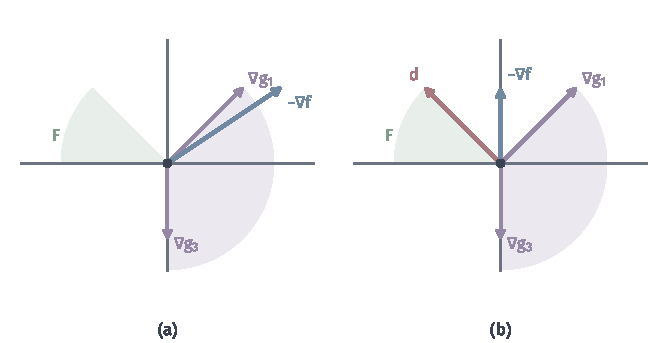
\includegraphics[width=112mm]{figures/05-optimization/06-constrained-optimization/matplotlib/kkt-farkas-cone/figure.pdf}
  \caption{Farkas引理的两种情形，画在方向空间中。紫色楔形是活动梯度张成的锥，浅绿楔形是线性化锥$\bm{F}$，蓝色箭头是$-\nabla f$。(a)$\tau=1/2$的角点：$-\nabla f=(3/2,1)$在锥内。(b)$\tau=2$的角点$(2,0)$：$-\nabla f=(0,1)$在锥外，红色箭头$\bm{d}=(-1,1)$在$\bm{F}$内，与负梯度成锐角，是下降方向。}
  \label{fig:kkt-farkas-cone}
\end{BookInlineFigure}

\paragraph{KKT条件}
式~\eqref{eq:kkt-farkas-stationary}只对活动约束求和。为了不必事先知道哪些约束活动，给每个不等式都配一个乘子，定义完整的Lagrange函数
\begin{equation}
 \mathcal{L}(\bm{x},\bm{\lambda},\bm{\nu})=f(\bm{x})+\sum_{i=1}^m\lambda_ig_i(\bm{x})+\sum_{j=1}^p\nu_jh_j(\bm{x}),
 \label{eq:kkt-lagrangian}
\end{equation}
并用乘积$\lambda_ig_i=0$规定“不活动的约束乘子为零”。这样就得到下面四组条件。

\begin{definition}[KKT条件]
\label{def:kkt-conditions}
设$f$、$g_i$、$h_j$在$\bm{x}^\star$处可微。若存在$\bm{\lambda}^\star\in\mathbb{R}^m$、$\bm{\nu}^\star\in\mathbb{R}^p$，使
\begin{align}
 &\nabla_{\bm{x}}\mathcal{L}(\bm{x}^\star,\bm{\lambda}^\star,\bm{\nu}^\star)=\bm{0}, \label{eq:kkt-stationarity}\\
 &g_i(\bm{x}^\star)\leq0,\quad h_j(\bm{x}^\star)=0, \label{eq:kkt-primal}\\
 &\lambda_i^\star\geq0, \label{eq:kkt-dual}\\
 &\lambda_i^\star g_i(\bm{x}^\star)=0, \label{eq:kkt-complementarity}
\end{align}
对所有$i=1,\ldots,m$，$j=1,\ldots,p$成立，就称$\bm{x}^\star$满足\term{KKT条件}（Karush--Kuhn--Tucker conditions），$(\bm{x}^\star,\bm{\lambda}^\star,\bm{\nu}^\star)$称为\term{KKT点}（KKT point），$(\bm{\lambda}^\star,\bm{\nu}^\star)$称为KKT乘子。
\end{definition}

表~\ref{tab:kkt-four-conditions}列出四组条件的分工。其中式~\eqref{eq:kkt-complementarity}称为互补松弛，它把活动集的选择藏进了乘积里。

\begin{BookInlineTable}
  \centering
  \begin{tabular}{@{}lll@{}}
    \toprule
    条件 & 式子 & 作用\\
    \midrule
    驻定 & \eqref{eq:kkt-stationarity} & 负梯度被约束的法向组合抵消\\
    原始可行 & \eqref{eq:kkt-primal} & 候选点满足全部约束\\
    乘子非负 & \eqref{eq:kkt-dual} & 墙只能推不能拉\\
    互补松弛 & \eqref{eq:kkt-complementarity} & 不活动约束不出力\\
    \bottomrule
  \end{tabular}
  \caption{KKT条件的四个组成部分。}
  \label{tab:kkt-four-conditions}
\end{BookInlineTable}

\paragraph{预算例的计算}
互补松弛把求解变成对活动集的枚举：猜一个活动集，令其余乘子为零，解方程，再检查可行性和符号。预算例的驻定条件是
\[
 x_1-2+\lambda_1-\lambda_2=0,\qquad x_2-1+\lambda_1-\lambda_3=0.
\]

取$\tau=2$。先猜没有活动约束，三个乘子都是零，得$\bm{x}=(2,1)$，但$g_1=1>0$，不可行。再猜只有$g_1$活动，$\lambda_2=\lambda_3=0$，$x_1+x_2=2$，由驻定条件得$x_1=2-\lambda_1$，$x_2=1-\lambda_1$，代入得
\[
 3-2\lambda_1=2,\qquad\lambda_1=\frac12,\qquad\bm{x}=\Bigl(\frac32,\frac12\Bigr).
\]
这一点可行，乘子非负，KKT条件全部成立。

取$\tau=1/2$。只有$g_1$活动时解出$\lambda_1=5/4$，$\bm{x}=(3/4,-1/4)$，不可行。再猜$g_1,g_3$活动，$x_2=0$，$x_1=1/2$，由第一个驻定方程得$\lambda_1=3/2$，第二个得$\lambda_3=\lambda_1-1=1/2$。全部条件成立。

让$\tau$连续变化，结果分三段：
\begin{equation}
 (\bm{x}^\star,\lambda_1,\lambda_3)=\begin{cases}
 \bigl((\tau,0),\ 2-\tau,\ 1-\tau\bigr),&0<\tau\leq1,\\
 \bigl((\tfrac{1+\tau}{2},\tfrac{\tau-1}{2}),\ \tfrac{3-\tau}{2},\ 0\bigr),&1\leq\tau\leq3,\\
 \bigl((2,1),\ 0,\ 0\bigr),&\tau\geq3,
 \end{cases}
 \label{eq:kkt-budget-solution}
\end{equation}
三段都有$\lambda_2=0$。图~\ref{fig:kkt-tau-regimes}画出最优点的轨迹和乘子曲线。

\begin{BookInlineFigure}
  \centering
  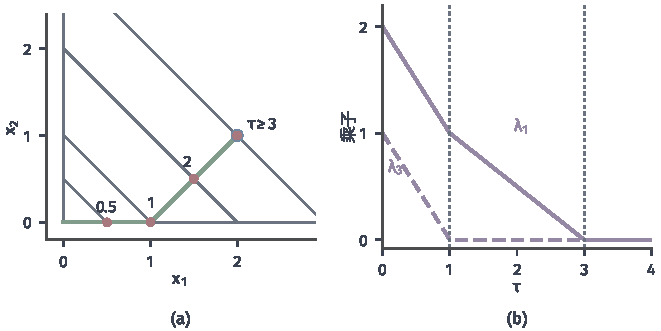
\includegraphics[width=112mm]{figures/05-optimization/06-constrained-optimization/matplotlib/kkt-tau-regimes/figure.pdf}
  \caption{预算例的解随$\tau$变化。(a)绿线是最优点轨迹，深灰细线是预算线$x_1+x_2=\tau$，红点对应$\tau=0.5,1,2,3$，空心点是$\bm{c}$。(b)乘子$\lambda_1$（实线）与$\lambda_3$（虚线），竖直虚线是活动集改变的位置$\tau=1,3$。}
  \label{fig:kkt-tau-regimes}
\end{BookInlineFigure}

这个例子说清了互补松弛的方向。$\lambda_i>0$推出约束活动，但约束活动推不出$\lambda_i>0$。$\tau=3$时预算线恰好经过$\bm{c}$，$g_1$活动，而$\lambda_1=0$：预算恰好够用，这堵墙碰到了点却不用出力。$\tau=1$时最优点是角点$(1,0)$，$g_3$活动，$\lambda_3=0$，同样如此。

从公式~\eqref{eq:kkt-budget-solution}还能再次看到影子价格。$1\leq\tau\leq3$时最优值是$(3-\tau)^2/4$，它对$\tau$的导数是$-(3-\tau)/2=-\lambda_1$：多一块钱，目标改善$\lambda_1$。

\subsection{乘子的存在与唯一性}
\label{sec:kkt-existence}

前面的推导把各步准备好了，现在把它们合起来。

\begin{theorem}[KKT条件的必要性]
\label{thm:kkt-necessary}
设$f$、$g_i$、$h_j$在局部最小点$\bm{x}^\star$附近连续可微。若$\bm{x}^\star$满足MFCQ，则存在KKT乘子$(\bm{\lambda}^\star,\bm{\nu}^\star)$，并且全体KKT乘子组成有界集合。若$\bm{x}^\star$满足LICQ，则KKT乘子唯一。
\end{theorem}

\begin{proof}
\emph{存在性。}由定理~\ref{thm:kkt-mfcq-exact}，切锥等于线性化锥。由定理~\ref{thm:kkt-tangent-necessary}，$\bm{F}(\bm{x}^\star)$中没有使$\langle\nabla f(\bm{x}^\star),\bm{d}\rangle<0$的方向。引理~\ref{lem:kkt-farkas}给出活动约束的乘子与$\bm{\nu}^\star$。不活动约束的乘子取零，四组条件全部成立。

\emph{有界性。}若乘子列$(\bm{\lambda}^{(k)},\bm{\nu}^{(k)})$的范数趋于无穷，把驻定方程除以这个范数，取收敛子列，极限$(\bar{\bm{\lambda}},\bar{\bm{\nu}})$的范数为$1$，满足$\bar{\bm{\lambda}}\geq\bm{0}$，不活动分量为零，并且
\[
 \sum_{i\in A(\bm{x}^\star)}\bar{\lambda}_i\nabla g_i(\bm{x}^\star)+\sum_{j=1}^p\bar{\nu}_j\nabla h_j(\bm{x}^\star)=\bm{0}.
\]

把上式与MFCQ的方向$\bar{\bm{d}}$作内积，等式项消失，得到
\[
 \sum_{i\in A(\bm{x}^\star)}\bar{\lambda}_i\langle\nabla g_i(\bm{x}^\star),\bar{\bm{d}}\rangle=0.
\]
每项都非正，而内积严格为负，所以$\bar{\bm{\lambda}}=\bm{0}$。剩下的等式项由$\nabla h_j$线性无关推出$\bar{\bm{\nu}}=\bm{0}$，与范数为$1$矛盾。

\emph{唯一性。}设有两组KKT乘子。不活动分量都是零，两个驻定方程相减，得到活动梯度和等式梯度的一个线性组合等于零，系数是两组乘子之差。LICQ说明系数全为零。
\end{proof}

由引理~\ref{lem:kkt-licq-implies-mfcq}，LICQ下存在性自动成立。全部活动约束与等式约束都是仿射函数时，$\bm{T}_{\bm{C}}=\bm{F}$不需要任何资格，乘子同样存在，只是有界性和唯一性不再有保证。

\paragraph{存在与唯一是两回事}
图~\ref{fig:kkt-multiplier-sets}对比几种情形的乘子集合。把预算线写两遍（$\tau=2$），MFCQ成立，驻定条件只约束$\lambda_1+\lambda_1'$的和，$\lambda_1+\lambda_1'=1/2$是一条线段：乘子存在、有界，但不唯一。

再看在$\{0\}$上最小化$x$。写成$x\leq0$，$-x\leq0$时，驻定方程是$1+\lambda_1-\lambda_2=0$，解集是无界射线，MFCQ不成立时有界性确实可能失去。写成$x=0$时，$\nu=-1$是唯一乘子。

\paragraph{没有乘子的最小点}
第三种写法最值得注意。最小化$x$，约束$g(x)=x^2\leq0$。可行集只有原点，所以$x^\star=0$是全局最小点。驻定方程是
\[
 1+\lambda\cdot2x^\star=1=0,
\]
对任何$\lambda$都无解，图~\ref{fig:kkt-multiplier-sets}(c)的残差恒为$1$。这是一个没有KKT乘子的最小点。

因此，不能仅凭驻定方程无解就排除一个候选点，除非已经确认它满足约束资格。这里的问题出在约束函数的写法上，$\nabla g(0)=0$让约束的一阶信息完全失效，与目标函数无关。

\begin{BookInlineFigure}
  \centering
  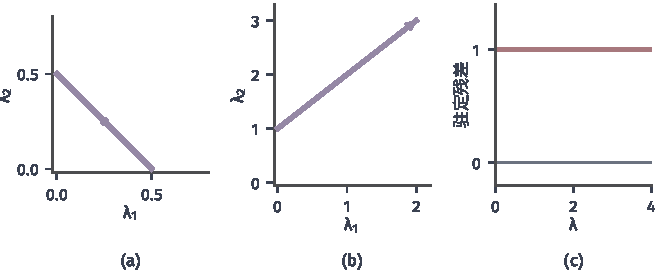
\includegraphics[width=112mm]{figures/05-optimization/06-constrained-optimization/matplotlib/kkt-multiplier-sets/figure.pdf}
  \caption{KKT乘子集合的三种情况。(a)预算线写两遍（$\tau=2$），乘子集合是线段$\lambda_1+\lambda_2=1/2$（这里$\lambda_2$表示重复约束的乘子），有界而不唯一。(b)$\min x$，约束$x\leq0$，$-x\leq0$：乘子集合是无界射线$\lambda_2=1+\lambda_1$。(c)$\min x$，约束$x^2\leq0$：对任何乘子，驻定残差都等于$1$，乘子不存在。}
  \label{fig:kkt-multiplier-sets}
\end{BookInlineFigure}

\subsection{凸问题的全局判别}
\label{sec:kkt-convex}

KKT条件在约束资格下是必要的，它能筛掉不合格的点，却不能确认合格的点就是最小点。什么时候能反过来？答案是问题凸的时候，而且这时连约束资格都不用检查。

\begin{theorem}[凸问题的KKT充分性]
\label{thm:kkt-convex-sufficient}
设$\bm{D}\subseteq\mathbb{R}^n$是包含可行集的开凸集，$f$与$g_i$在$\bm{D}$上凸且可微，$h_j$是仿射函数。若$(\bm{x}^\star,\bm{\lambda}^\star,\bm{\nu}^\star)$是KKT点，则$\bm{x}^\star$是问题~\eqref{eq:kkt-problem}的全局最小点。
\end{theorem}

\begin{proof}
任取可行点$\bm{x}$，记$\bm{u}=\bm{x}-\bm{x}^\star$。由第~\ref{chap:optimization}章的一阶支撑不等式，凸函数$f$满足
\[
 f(\bm{x})\geq f(\bm{x}^\star)+\langle\nabla f(\bm{x}^\star),\bm{u}\rangle.
\]
再由驻定条件~\eqref{eq:kkt-stationarity}，把梯度替换掉：
\[
 f(\bm{x})\geq f(\bm{x}^\star)-\sum_{i=1}^m\lambda_i^\star\langle\nabla g_i(\bm{x}^\star),\bm{u}\rangle-\sum_{j=1}^p\nu_j^\star\langle\nabla h_j(\bm{x}^\star),\bm{u}\rangle.
\]

$h_j$仿射，$\bm{x}$与$\bm{x}^\star$都可行，所以
\[
 \langle\nabla h_j(\bm{x}^\star),\bm{u}\rangle=h_j(\bm{x})-h_j(\bm{x}^\star)=0,
\]
最后一个和式消失。

对$\lambda_i^\star=0$的项，这一项本来就是零。对$\lambda_i^\star>0$的项，互补松弛给出$g_i(\bm{x}^\star)=0$，再对凸函数$g_i$用支撑不等式：
\[
 \langle\nabla g_i(\bm{x}^\star),\bm{u}\rangle\leq g_i(\bm{x})-g_i(\bm{x}^\star)=g_i(\bm{x})\leq0.
\]
所以和式中每一项$-\lambda_i^\star\langle\nabla g_i,\bm{u}\rangle$都非负，代回得到$f(\bm{x})\geq f(\bm{x}^\star)$。
\end{proof}

证明的每一步都用到了相应的假设：目标凸给出一个全局下界，$g_i$凸把梯度内积换成函数值，乘子非负保证不等号的方向，互补松弛消去$g_i(\bm{x}^\star)$，等式仿射让等式项消失。

把它用在预算例上。目标凸，约束都是仿射函数，所以式~\eqref{eq:kkt-budget-solution}中的点都是全局最小点，这一步不需要再检查什么。

还可以从Lagrange函数看这个结论。固定乘子后，$\mathcal{L}(\cdot,\bm{\lambda}^\star,\bm{\nu}^\star)$是凸函数，驻定点就是它的全局最小点。在可行点上$\mathcal{L}\leq f$，在$\bm{x}^\star$处两者相等，于是目标在$\bm{x}^\star$被一个碗从下面托住了。图~\ref{fig:kkt-convex-vs-nonconvex}(a)取最小化$(x-2)^2$、约束$x-1\leq0$的问题，$x^\star=1$，$\lambda^\star=2$，$\mathcal{L}(x,2)=(x-1)^2+1$就是紫色的碗，可行域上它在$f$的下方。

\begin{BookInlineFigure}
  \centering
  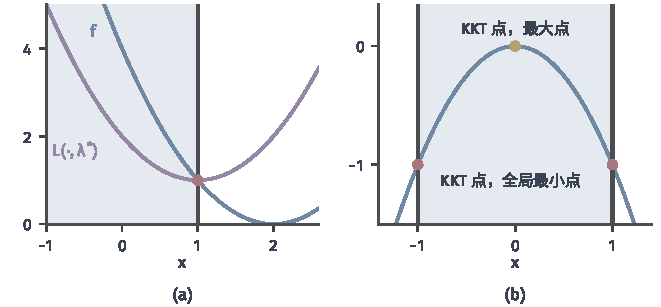
\includegraphics[width=112mm]{figures/05-optimization/06-constrained-optimization/matplotlib/kkt-convex-vs-nonconvex/figure.pdf}
  \caption{凸与非凸问题中的KKT点。浅蓝带是可行域，深灰线是活动约束的位置。(a)$\min(x-2)^2$，$x\leq1$：KKT点$x^\star=1$（红），$\lambda^\star=2$。紫色曲线$\mathcal{L}(x,2)=(x-1)^2+1$在可行域上位于$f$（蓝）下方，并在$x^\star$处与$f$相接。(b)$\min-x^2$，$\lvert x\rvert\leq1$：三个KKT点中$x=0$（黄）是最大点，$x=\pm1$（红）是全局最小点。}
  \label{fig:kkt-convex-vs-nonconvex}
\end{BookInlineFigure}

\paragraph{去掉凸性会怎样}
一般非凸问题中，KKT条件只提供候选。在$[-1,1]$上最小化$-x^2$，约束写成$x-1\leq0$，$-x-1\leq0$。点$x=0$没有活动约束，$f'(0)=0$，乘子取零就满足KKT条件，但它是全局最大点。点$x=1$处由$-2+\lambda_1=0$得$\lambda_1=2$，也满足KKT条件，它才是最小点。KKT方程分不开这两种点，见图~\ref{fig:kkt-convex-vs-nonconvex}(b)。

等式必须是仿射函数也不是多余的要求。单位圆周的$h(\bm{x})=x_1^2+x_2^2-1$是凸函数，目标$\frac12\lVert\bm{x}-(2,0)\rVert_2^2$也是凸函数，但$(-1,0)$是KKT点，却是圆周上的全局最大点。$h=0$的解集不是凸集，定理的证明在处理等式项那一步就失效了。

另外，充分性不提供存在性。$\min x$，$x^2\leq0$是凸问题，最小点却没有KKT乘子。表~\ref{tab:kkt-necessity-sufficiency}把必要性与充分性的条件放在一起。

\begin{BookInlineTable}
  \centering
  \begin{tabular}{@{}lll@{}}
    \toprule
    结论方向 & 所需条件 & 结论\\
    \midrule
    局部最小$\Rightarrow$KKT & MFCQ（或LICQ、仿射约束） & 存在乘子\\
    KKT$\Rightarrow$全局最小 & 目标、$g_i$凸，$h_j$仿射 & 不需要约束资格\\
    KKT$\Rightarrow$局部最小 & 一般不成立 & 需要二阶条件\\
    \bottomrule
  \end{tabular}
  \caption{KKT条件的必要性与充分性。}
  \label{tab:kkt-necessity-sufficiency}
\end{BookInlineTable}
